\chapter{Limited Proteolysis}
\label{chap:limprot}

The module Limited Proteolysis is designed to post-process the results from an enzymatic
digestion performed in two steps. The first step is assumed to be a limited proteolysis
in which a large protein is split in smaller fragments. The fragments are then separated
using a SDS-PAGE electrophoresis. Finally, selected bands from the gel are submitted to
a full enzymatic digestion and the generated peptides are analyzed using mass spectrometry.

The main objective of the module is to identify the protein fragments generated in
the initial limited proteolysis from the peptides found in the MS analyzed gel spots.
This is achieved by performing an equivalence test\cite{Limentani2005a} between the
peptides in the selected gel spots and a positive control spot containing the full length
Target protein. In this way, peptides leaked from one gel spot to another can be
eliminated. Several replicates of the experiment are expected.

\section{Definitions}
\label{sec:limprotDefinitions}

Before explaining in detail the interface of the module and how does the module
work, let's make clear the meaning of some terms that will be used in the following
paragraphs.

\phantomsection
\begin{itemize}
    \item \textit{Recombinant protein}: actual amino acid sequence used in the mass
    spectrometry experiments. It may be identical to the native sequence of the Target
    protein under study or not.
    \item \textit{Native protein}: full amino acid sequence expressed in wild type cells.
    \item \textit{Detected peptide}: any peptide detected in any of the MS
    experiments including the control experiments.
    \item \textit{Relevant peptide}: a detected peptide with a Score value above
    a user-defined threshold, see page \pageref{par:limprotScoreValue}.
    \item \textit{Filtered peptide}: a relevant peptide with equivalent intensities
    in the control and a given gel spot at the chosen significance level.\label{par:limprotFP}
    \item \textit{Fragment}: group of filtered peptides with no gaps when their
    sequences are aligned to the sequence of the recombinant/native protein.
\end{itemize}

For example, there are three fragments in the alignment shown below. The first fragment
is formed by sequences \numrange{1}{3} since there is no gap in the sequence MKKTAIAIAVAL.
SEQ\num{4} forms the second fragment because there is a gap between the last residue
in SEQ\num{3} and the first residue in SEQ\num{4} and another gap between the last
residue in SEQ\num{4} and the first residue in SEQ\num{5}. For the same reason
SEQ\num{5} forms the third fragment.

\begin{texshade}{./TeX_files/test.fasta}
    \residuesperline*{50}
    \shadingmode[kenny]{functional}
    \hideconsensus
\end{texshade}

\section{The input files}

The Limited Proteolysis module requires a Data file containing the detected peptides
and a sequence file containing the amino acid sequence of the recombinant protein
used in the study. Both files must follow the guidelines specified in \autoref{sec:dataFile}.
In short, the Data file must have a tabular format with tab separated columns and
the name of the columns are expected as first row. The Sequence file is expected
to contain at least one sequence and to be FASTA formatted. If more than one sequence
is found in the Sequence file the first sequence will be taken as the sequence of
the Recombinant protein and the second sequence will be taken as the sequence of
the Native protein. All other sequences are discarded.

\section{The interface}

The tab of module Limited Proteolysis is divided in two regions (\autoref{fig:limprotTab}).

\begin{figure}[h]
    \centering
    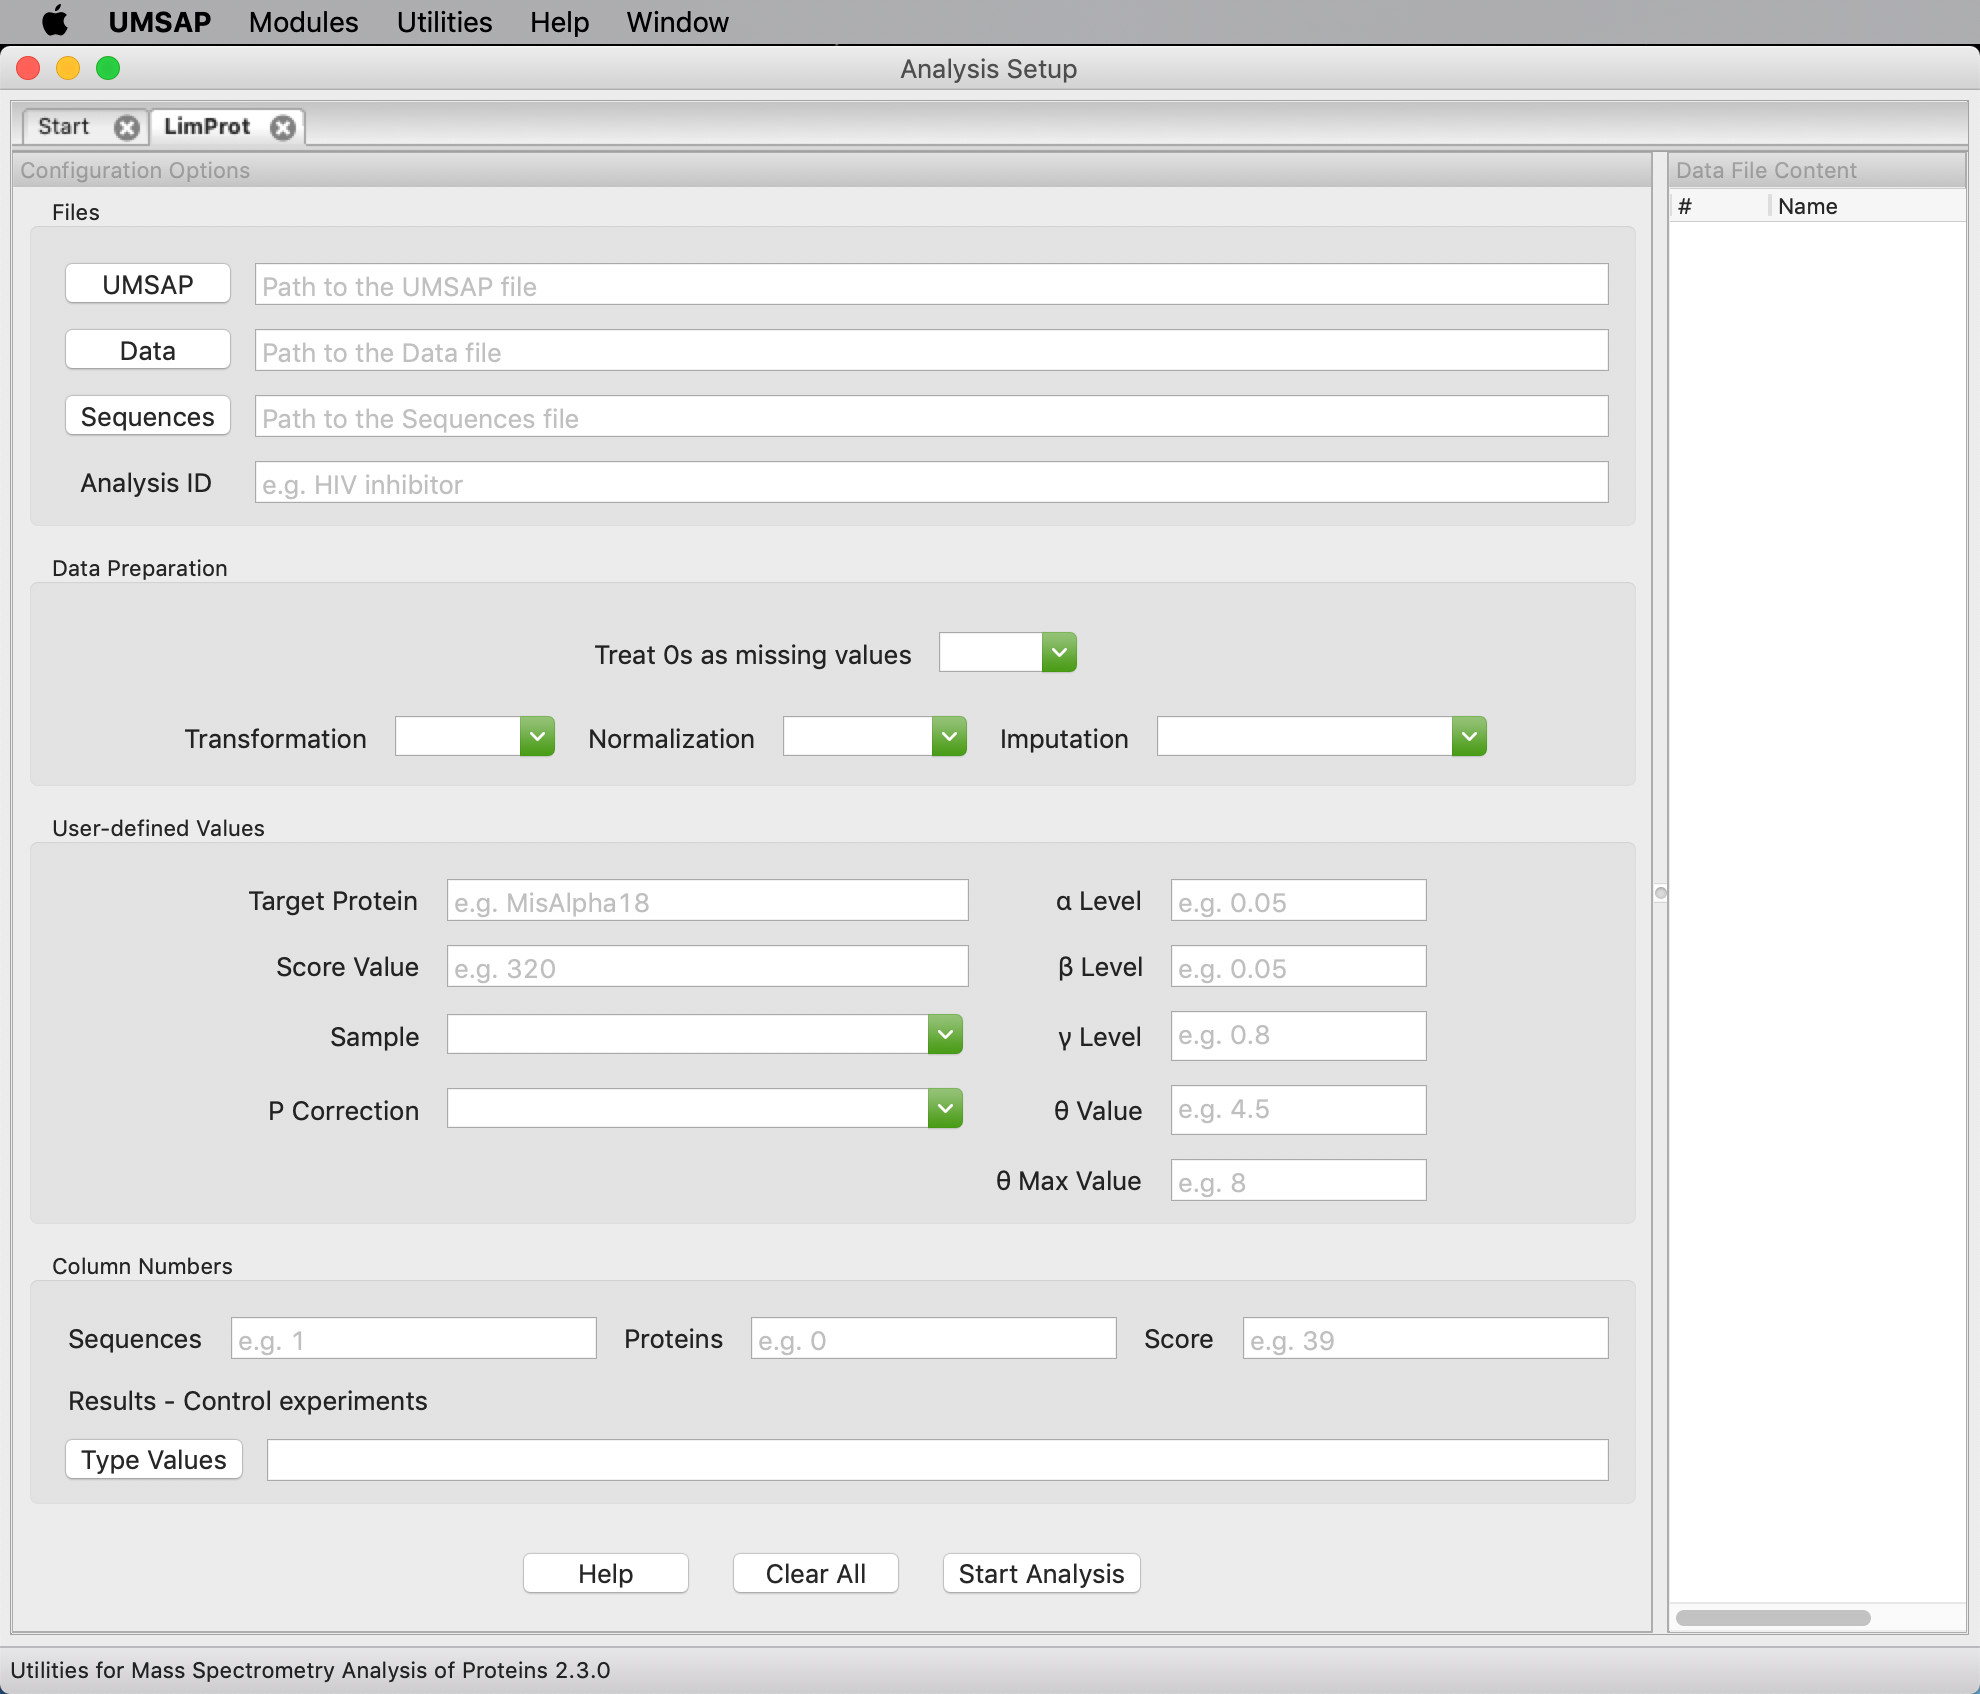
\includegraphics[width=0.7\textwidth]{./IMAGES/MOD-LIMPROT/limprot-mod.jpg}
    \caption[The Limited Proteolysis module tab]{\textbf{The Limited Proteolysis
    module tab.} This tab allows users to perform the analysis of the results obtained
    during a two steps enzymatic proteolysis experiment where the products from the
    first limited digestions are separated using SDS-PAGE electrophoresis.}
    \label{fig:limprotTab}
    \vspace{-5pt}
\end{figure}

Region Data File Content holds a table to show the number and name of the columns in
the selected Data file. The table will be automatically filled after selecting the
file. Selected rows in the table can be copied (Cmd+C) and pasted (Cmd+V) to the
text fields in region Configuration Options.

Region Configuration Options contains all the fields needed to configure and
run the analysis.

Section Files contains three buttons and a text field. Here users select the input
and output files for the analysis.

\num{1}. The button UMSAP allows selecting the location
and name of the umsap file. When selecting an already existing umsap file the operating
system will ask if it is ok to replace the file, the answer can be yes since UMSAP
will never overwrite or replace an umsap file. Instead, the new analysis will be
added to the already existing file. Only umsap files can be selected here.

\num{2}. The button Data allows selecting the input
data file that will be used for the analysis. The Data file is expected to be a
plain text file with tab separated columns and the name of the columns in the first
row of the file. Only .txt files can be selected here.

\num{3}. The button Sequences allows selecting the
FASTA file containing the sequence of the Recombinant protein and the Native protein.
The FASTA file must contain at least one sequence.

\num{4}. The text field Analysis ID allows providing an ID for the analysis
to be run. The date and time of the analysis will be automatically added to the
beginning of the name. For example, the Analysis ID \textit{First experiment} will
be transformed into \textit{20220504-124534 - First experiment}.

Section Data Preparation contains four dropdown boxes. Here users select how the data
in the Data file should be prepared before starting the analysis (\autoref{chap:dataPrep}).

\num{1}. The dropdown Treat \num{0}s as missing values allows defining how
to handle zero values present in the Data file. Selecting Yes results in UMSAP
replacing zero values with NA values. Selecting No results in UMSAP considering
zeros as valid values.

\num{2}. The dropdown Transformation allows selecting the Transformation method
to be applied to the data.

\num{3}. The dropdown Normalization allows selecting the Normalization method
to be applied to the data.

\num{4}. The dropdown Imputation allows selecting the Imputation method used
to replace missing values in the data.

Section User-defined values contains seven text fields and one dropdown box. Here
users configure the Limited Proteolysis analysis to be run.

\phantomsection
\num{1}. The text field Target Protein\label{par:limprotTargetProtein} allows
specifying the protein of interest. Users may type here any unique protein identifier
present in the Data file. The search for the Target Protein is case-sensitive, meaning
that eFeB is not the same as efeb.

\phantomsection
\num{2}. The text field Score Value\label{par:limprotScoreValue} allows
defining a threshold value above which the detected peptides will be considered as
relevant. The Score Value is an indicator of how reliable was the detection of the peptide
during the MS experiments. The value given to UMSAP depends on the program generating
the Data file. Only one real number equal or greater than zero will be accepted here.
A value of zero means all detected peptides belonging to the Target Protein will
be treated as relevant peptides.

\num{3}. The dropdown Samples allows specifying whether samples are independent
or paired. For example, samples are paired when the same Petri dish is used for the
control and experiments.

\numrange[range-phrase = --]{4}{8}. The text fields $\alpha$, $\beta$, $\gamma$,
$\Theta$ and $\Theta$max are used to configure the equivalence test \cite{Limentani2005a}
performed to identify peptides in the selected gel spots with equivalent intensity
values to the control spots (\autoref{sec:limprotEquivalenceTest}). $\alpha$, $\beta$ and 
$\gamma$ must be between \num{0} and \num{1}. The value of $\Theta$ is optional. If
left blank, then UMSAP will calculate a value for each peptide based on the intensity values
found in the Data file. If given, then the given value will be used for each peptide.
$\Theta$max is the maximum value to consider the intensity values in the gel spot
and control as equivalent.

Section Column numbers contains four text fields. Here, users provide the column
numbers in the Data file from where UMSAP will get the information needed to perform
the Limited Proteolysis analysis. All columns specified in this section must be present
in the Data file. Column numbers start at \num{0}. The column numbers are shown in
the table of Region Data File Content after the Data file is selected.

\num{1}. The text field Sequences allows defining the column in the Data
file containing the sequences of the peptides identified in the MS experiments.
Only one integer number equal or greater than zero will be accepted here.

\num{2}. The text field Detected Proteins allows defining the column in
the Data file containing the unique protein identifier for the proteins detected
in the MS experiments. It is in this column where the program will look for the
Target Protein value given in Section User-defined values. It is important that
in this column the Target Protein value is used to identify only one protein. Only
one integer number equal or greater than zero will be accepted here.

\num{3}. The text field Score allows defining the column in the Data file
containing the Score values. It is in this column where the program will look for
the values to be compared against the Score threshold given in Section User-defined
values.

\phantomsection
\num{4}. \label{par:limprotResultControl}The text field Results - Control experiments
allows defining the columns in the Data file containing the results of the
control and experiments. The button Type Values calls a helper window
(\autoref{fig:limprotResControlWindow}) where users can type the information needed. 

\begin{figure}[h]
    \centering
    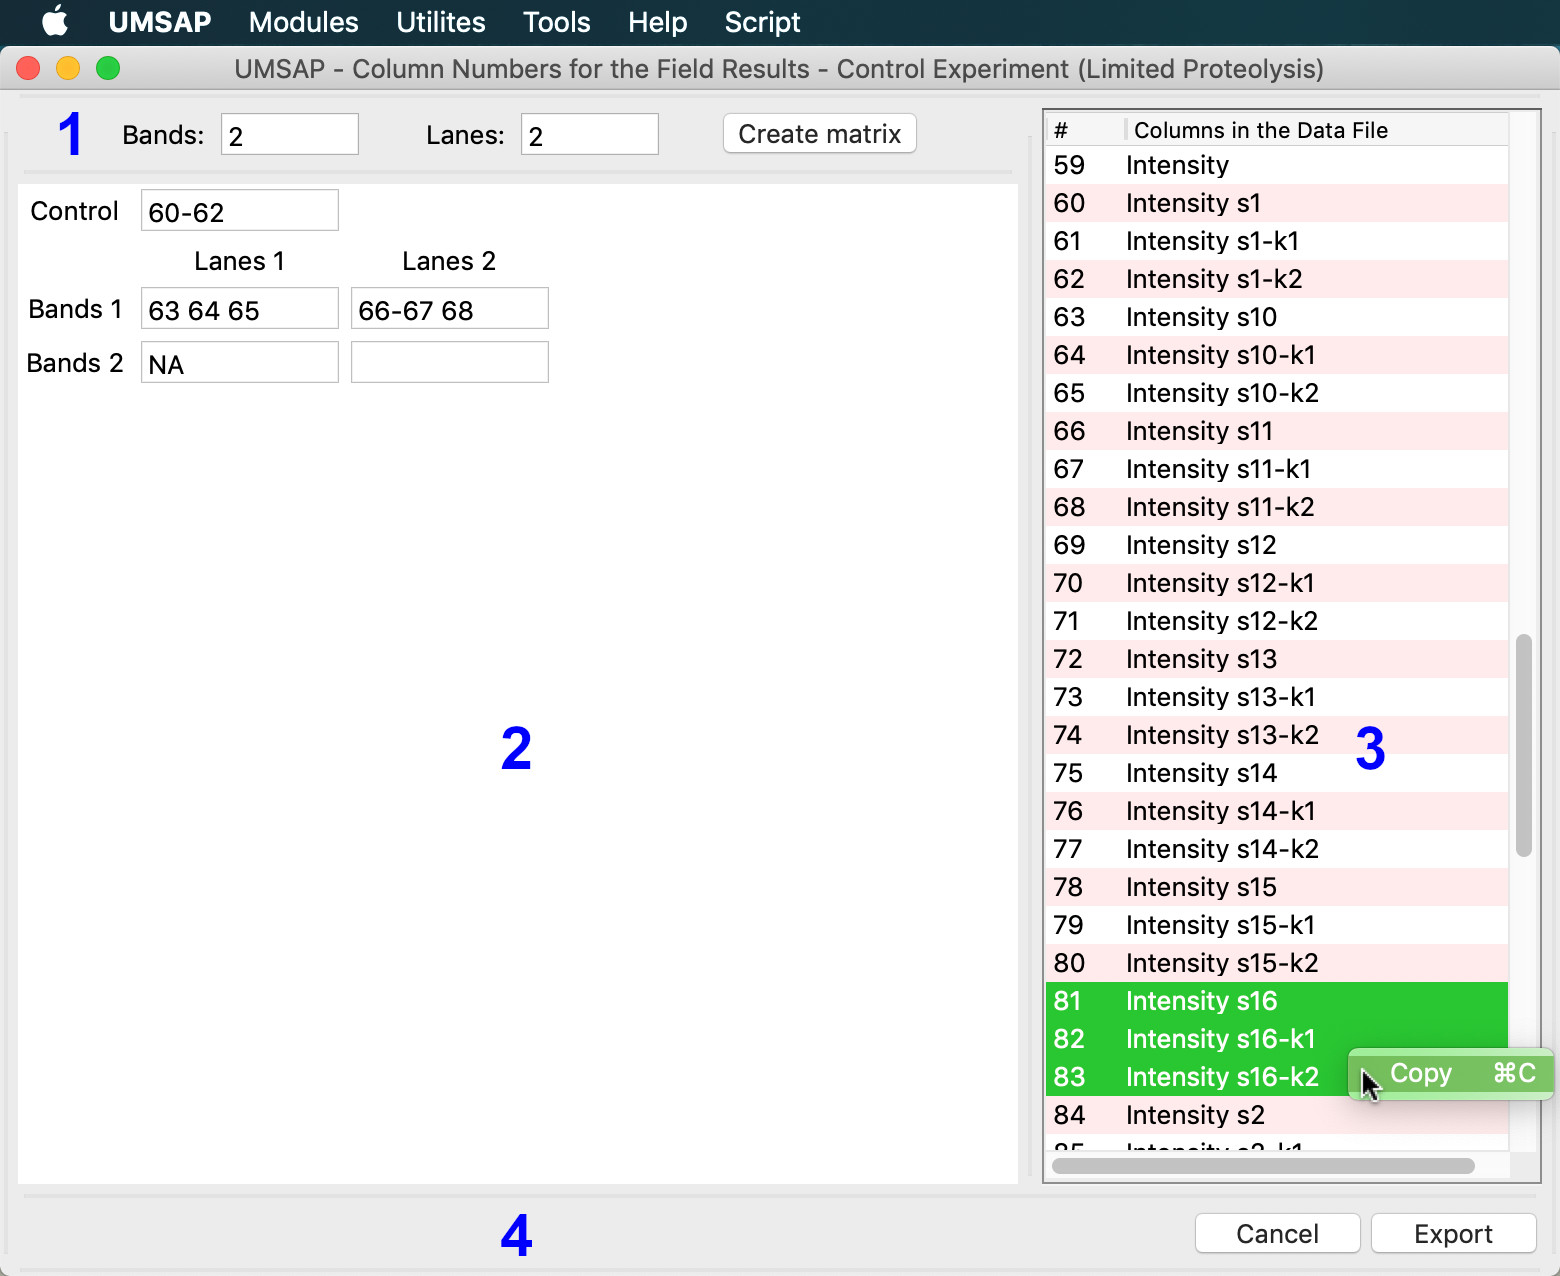
\includegraphics[width=0.7\textwidth]{./IMAGES/MOD-LIMPROT/limprot-rescontrol.jpg}
    \caption[The Result - Control experiments helper window]{\textbf{The Result -
    Control experiments helper window.} This window allows typing the column
    numbers in the Data file containing the MS results for the selected gel spots.} 
    \label{fig:limprotResControlWindow}
    \vspace{-5pt} 	
\end{figure}

The helper window is divided in two Regions. Region Data File Content will show the 
number and name of the columns present in the selected Data file. Region
Configuration Options has two sections. The upper section allows defining the number
of bands and lanes of interest in the gel as well as the label for lanes, bands and
control spot. The button Setup Fields creates the corresponding text fields in the
bottom section to type the column numbers. Each text field should contain the column
numbers with the MS results for the given gel spot. The values for the text fields
should be positive integer numbers or a range of integers, e.g. 
\numrange[range-phrase=--]{60}{62} or left blank for empty gel spots. Selected rows
in the table can be copied (Cmd+C) and then pasted (Cmd+V) in the text fields. 
Duplicate column numbers are not allowed. 

\section{The analysis}
\label{sec:limprotEquivalenceTest}
First, UMSAP will check the validity of the user-provided input and then the selected
Data file is read. The columns specified in section Column numbers are extracted
from the Data file. All other columns present in the Data file are discarded. After
this, all steps selected in the Data Preparation section are applied to the columns
specified in the text field Result - Control experiments (\autoref{chap:dataPrep}).
Then, the following actions are performed.

All rows in the prepared data containing peptides that do not belong to the Target
Protein are removed. Then, all rows containing peptides from the Target Protein
but with Score values lower than the user-defined Score threshold are removed. These
steps leave only relevant peptides, this means, peptides with a Score value higher
than the user-defined threshold that belong to the Target Protein. For each one of
these relevant peptides the equivalence test is performed \cite{Limentani2005a}.

The implementation of the equivalence test is based on the following equations:
\begin{equation}
    \label{eq:limprotDeviationUpperLimit}
    s^* = s\sqrt{\frac{n-1}{\chi^2_{(\gamma, n-1)}}}
\end{equation}
\begin{equation}
\label{eq:limprotAcceptanceCriterion}
\Theta = \delta + s^*\left[t_{(1-\alpha, 2n-2)} + t_{(1-\beta/2, 2n-2)}\right]\sqrt{\frac{2}{n}}
\end{equation}
\begin{equation}
\label{eq:limprotEquivalenceTest}
(\bar{y}_1 - \bar{y}_2) \pm t_{(1-\alpha, n_1+n_2-2)} \cdot \sqrt{s^2_p\left(\frac{1}{n_1}+\frac{1}{n_2}\right)}
\end{equation}

where $s^*$ is an estimate of the upper confidence limit of the standard deviation,
$\chi^2_{(\gamma, n-1)}$ is the ($100\gamma$)th percentile of the chi-squared distribution
with $n-1$ degrees of freedom, $\Theta$ is the acceptance criterion, $\delta$ is the
absolute value of the true difference between the group's mean values, $t$ is the
Student's $t$ value, $\bar{y}$ is the measurement mean and $s_p$ is the pooled standard
deviation of the measurements calculated with:
\begin{equation}
\label{eq:poolStDev}
s_p =  \sqrt{\frac{(n_1-1)s^2_1+(n_2-1)s^2_2}{n_1+n_2-2}}
\end{equation}
$\alpha$, $\beta$, $\gamma$ and $\Theta$ are the parameters defined in section
User-defined values of region Configuration Options in the tab of the module.

In essence, for each relevant peptide, the control experiments are used to estimate
the upper confidence limit for the standard deviation using \autoref{eq:limprotDeviationUpperLimit}
and then the acceptance criterion is calculated with \autoref{eq:limprotAcceptanceCriterion}.
Finally, the confidence interval for the mean difference for the gel spot and the
control is calculated with \autoref{eq:limprotEquivalenceTest} and compare to $\Theta$.
Peptides with equivalent mean intensity in at least one gel spot and the control
are retained while not equivalent peptides are discarded.

If the value of $\Theta$ is given in section User-defined values of the module's tab
then only the confidence interval for the mean difference is calculated, and the value
is directly compared to the given $\Theta$ value. The maximum possible $\Theta$ value
must always be provided. The reason for this is that when only a few replicates of the
experiments are performed the calculated $\Theta$ value may be too large and then
the equivalence test is easily past by all relevant peptides.

After the filtered peptide (FP) are identified the modules creates the output files.

\section{The results window}

The window showing the results from a Limited Proteolysis analysis is divided in
four regions (\autoref{fig:limprotResWindow}).

\begin{figure}[h]
    \centering
    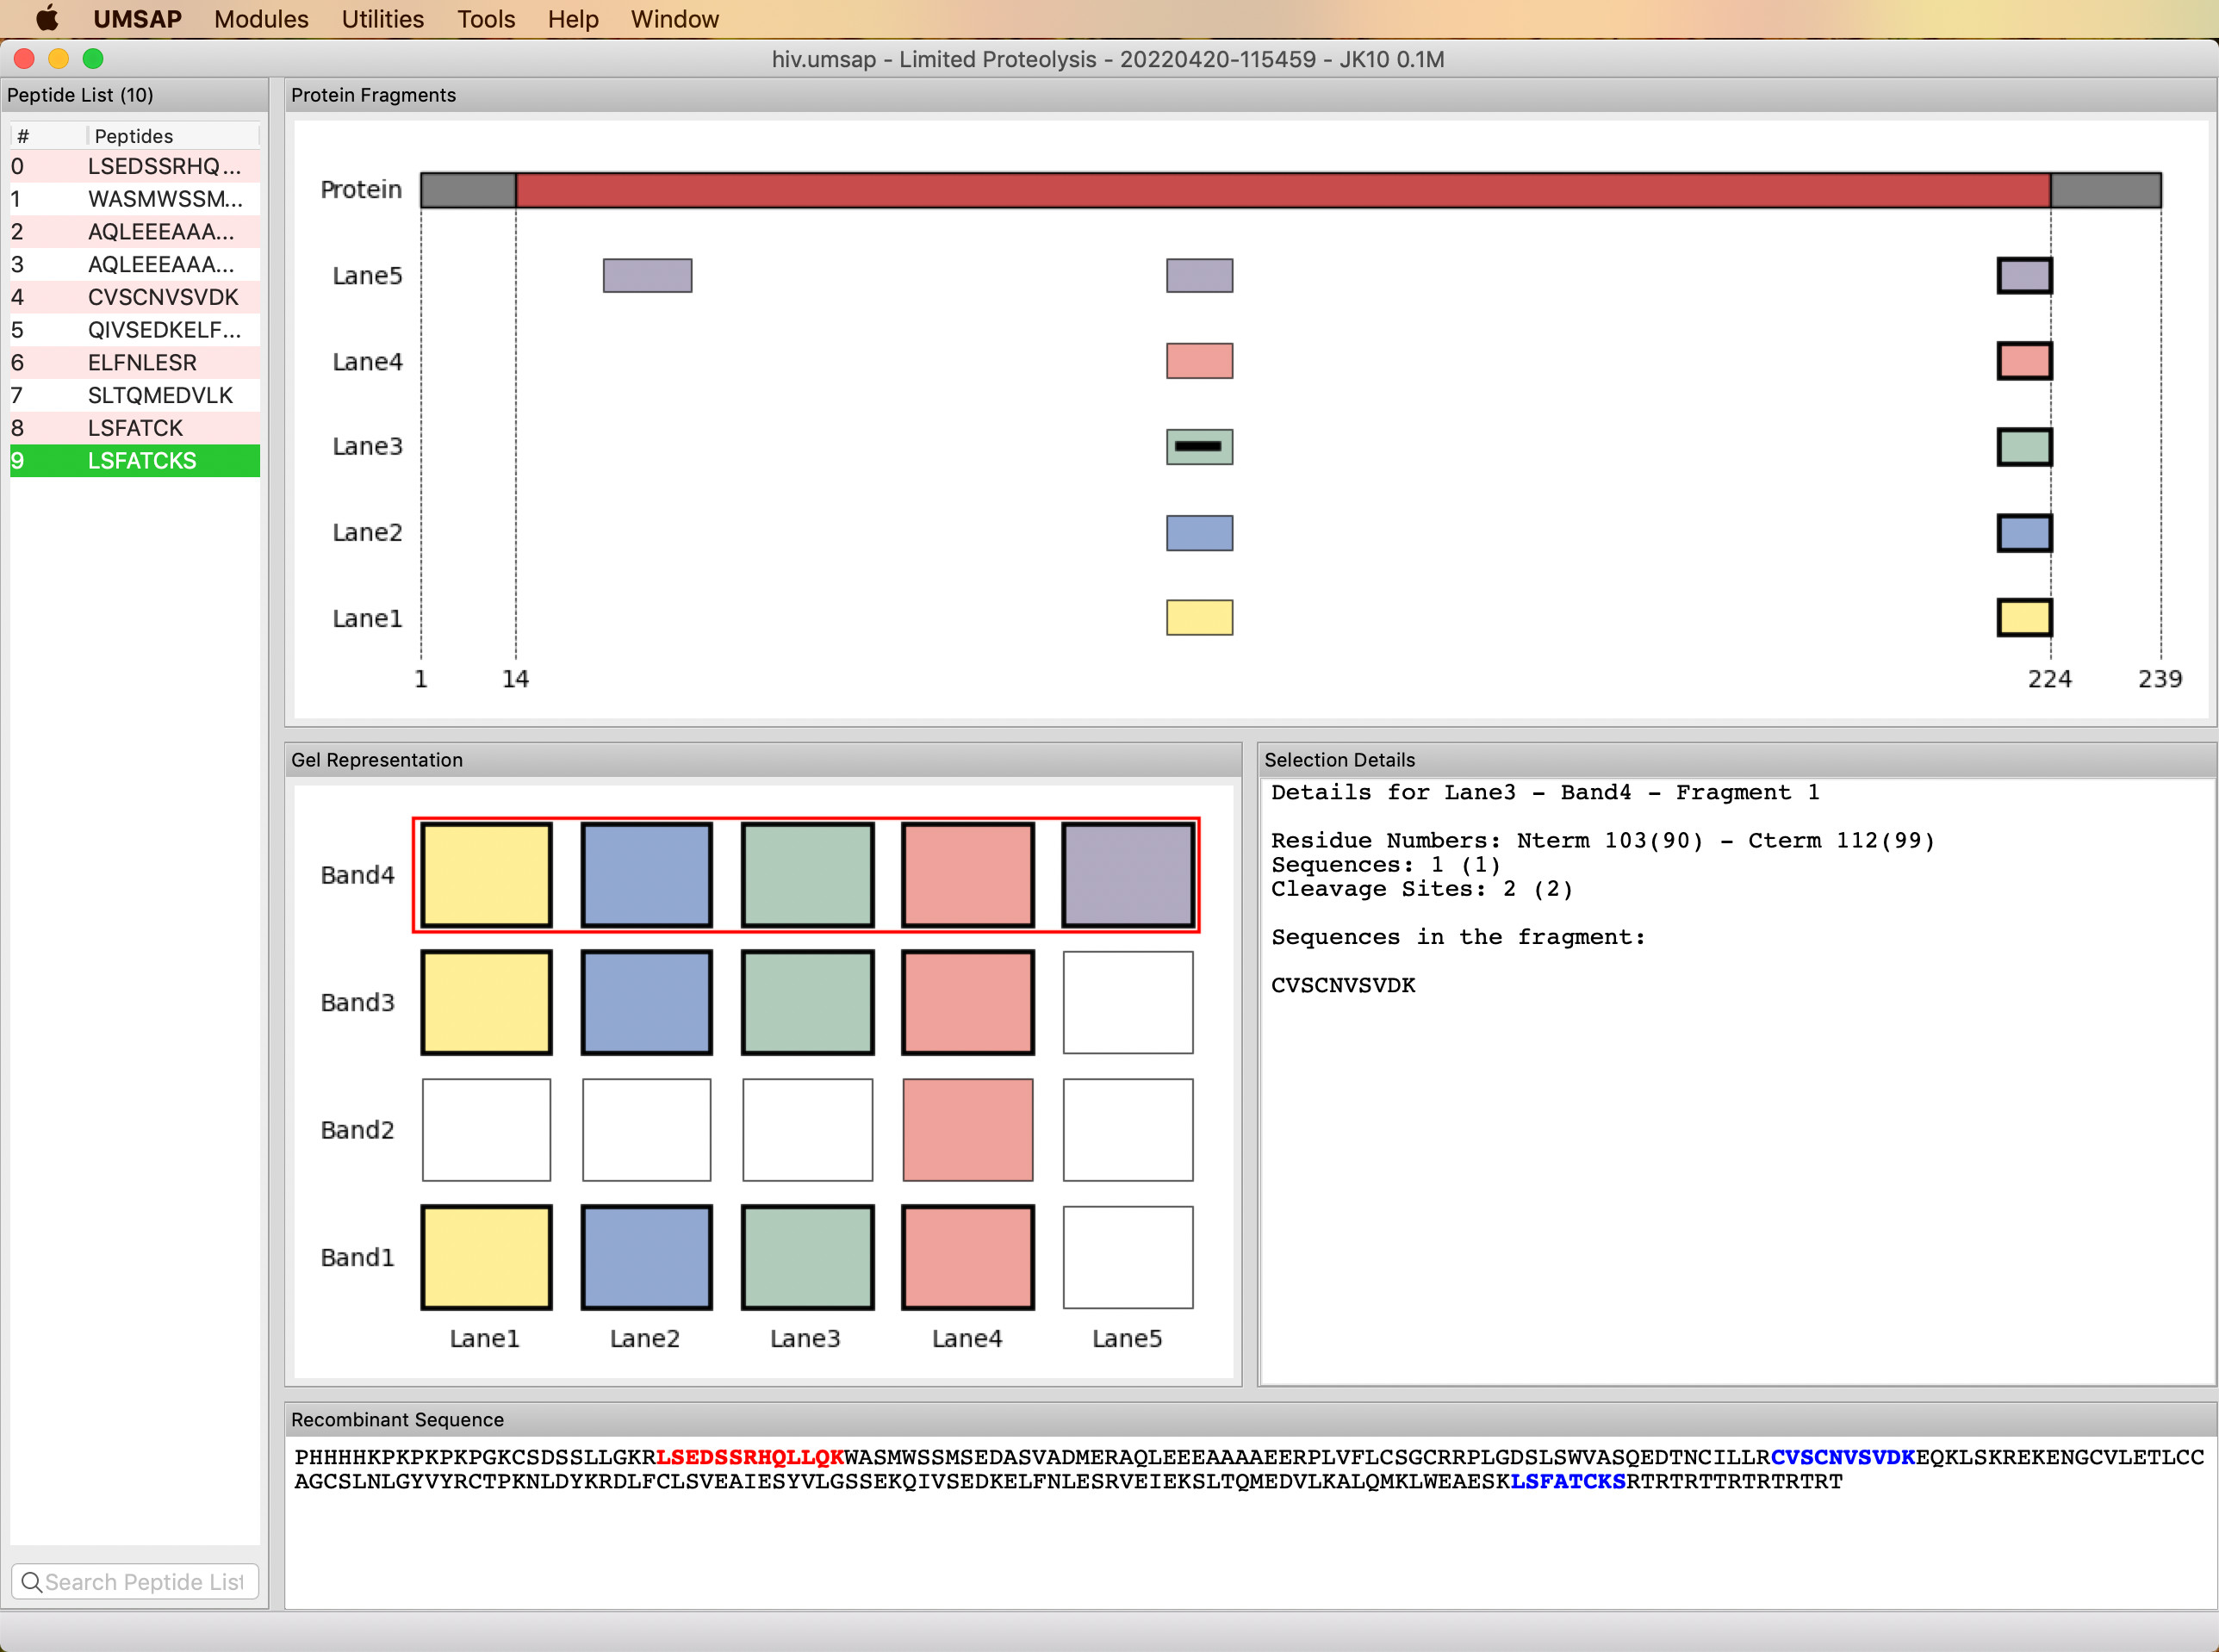
\includegraphics[width=0.8\textwidth]{./IMAGES/MOD-LIMPROT/limprot-res.jpg}
    \caption[The Limited Proteolysis result window]{\textbf{The Limited Proteolysis
    result window.} Users can perform here the analysis of the fragments obtained
    in the Limited Proteolysis experiments.}
    \label{fig:limprotResWindow}
    \vspace{-5pt}
\end{figure}

Region Peptide List contains a table with all FP detected during the analysis. Selecting
a peptide in the table will highlight with a thick black border all gel spot in
Region Gel Representation and all fragments in region Protein Fragments where the
selected peptide was found. In addition, region Recombinant Sequence will show the
selected peptide in blue. The search box at the bottom allows searching for a sequence
in the list of FP.

Region Gel Representation contains a representation of the analyzed gel. Here, each
gel spot is represented with a square. White squares represent gel spot for which
no peptide from the Target Protein was detected with intensity values equivalent
to the controls or that were not analyzed because no column number information was
given when configuring the analysis. The rest of the square will be colored according
to the band/lane they belong to.

There are two selection modes available for region Gel Representation. In the Lane
selection mode a left click over an empty space in the gel representation will select
the closer lane. In this mode the gel spot will be colored according to the band
they belong to. The selected lane will be highlighted with a red rectangle. The band
selection mode works similarly, but users can select bands and the gel spot are colored
according to the lane they belong to. The selection mode can be toggled through
the menu Tools (Cmd+L). In addition, the entire gel can be
selected (Cmd+A) or a single gel spot can be selected with a left click. Any selection
on the gel will update the content of Regions Protein Fragments, Selection Details
and Recombinant Sequence.

Region Protein Fragments will display a graphical representation of the fragments
found in each gel spot for the selected band/lane. The first fragment in this region
represents the full length of the recombinant sequence of the Target Protein. Here
the central red section represents the sequence in the recombinant protein that is
identical to the native protein sequence while gray sections represent the sequences
in the recombinant protein that are different to the native protein sequence. If
the sequence of the native protein was not given then the fragment is shown in gray.
The fragments are color coded using the same colors of the band/lane they belong to.
Selecting a fragment will update the information shown in regions Selection Details
and Recombinant Sequence.

Region Selection Details will show information about the selected lane/band, gel
spot in region Gel Representation or the selected fragment in region Protein Fragments.
The displayed information for a selected band/lane includes the number of non-empty
lanes/bands, the number of fragments identified in each non-empty gel spot in the
band/lane and the protein regions identified. Selecting a gel spot will display this
information only for the gel spot. Selecting a fragment in region Protein Fragments
will display the following information: number of cleavage sites, first and last
residue number for the selected fragment and a sequence alignment of all peptides
forming the fragment.

Region Recombinant Sequence shows the residues in the recombinant protein with gray
letters. Selecting a peptide in region Peptide List or a fragment in region Protein
Fragments or a gel spot in region Gel Representation will highlight the sequence of the
peptides in the selection using blue letters. Selecting a band/lane or the whole gel
will highlight the sequence of the peptides in the selection using red letters.

\section{The Tools menu}
\label{sec:limprotToolsMenu}

The menu Tools in the window showing the results from a Limited Proteolysis analysis
allows viewing any of the analyses contained in the selected umsap file. Users
can toggle the band/lane selection mode (Cmd+L) and select all gel spot in the analysis
(Cmd+A). In addition, the zoom level in the plots can be reset (Shift+Alt+Z) and
an image of the plots can be created (Shift+Alt+I).

The submenu Clear Selection allows removing any selection done by the user. In
particular, the entry All (Cmd+K) will remove all selections basically resetting
the state of the window.

The menu Tools also allows duplicating the window (Cmd+D) for easier comparison of
two or more analysis, checking the Data Preparation steps of the analysis (Cmd+P),
exporting the results of the analysis to a tab separated CSV file (Cmd+E) and to
export the sequence alignments (Cmd+S) between the peptides found in the analysis
and the sequence of the recombinant protein.